\chapter{Cryptocurrencies}

There were hundreds of failed attempts of creating cryptographic payment systems before cryptocurrencies like Bitcoin and Ethereum come into existence. Some of these systems are listed in figure \ref{paymentSystems}. All of them were created before Bitcoin, and despite that, some of these attempts were only academic proposals, others were actually deployed and tested systems, only a few of them survived to these days. One of the survival is PayPal, but only because it quickly give up its original idea of hand-held devices for cryptographic payments.\cite{wayner1997digital}

So there is a question, what makes cryptocurrencies successful nowadays?  It may be it's easy to use principle and no need for external hardware. 
Another critical component of cryptocurrencies discussed in this work is Blockchain. Simply, it is a ledger in which are all transactions securely stored. The idea behind blockchains is pretty old, and it was originally used for timestamping digital documents.\cite{haber1990time} 


\begin{figure}[H]
    \centering
    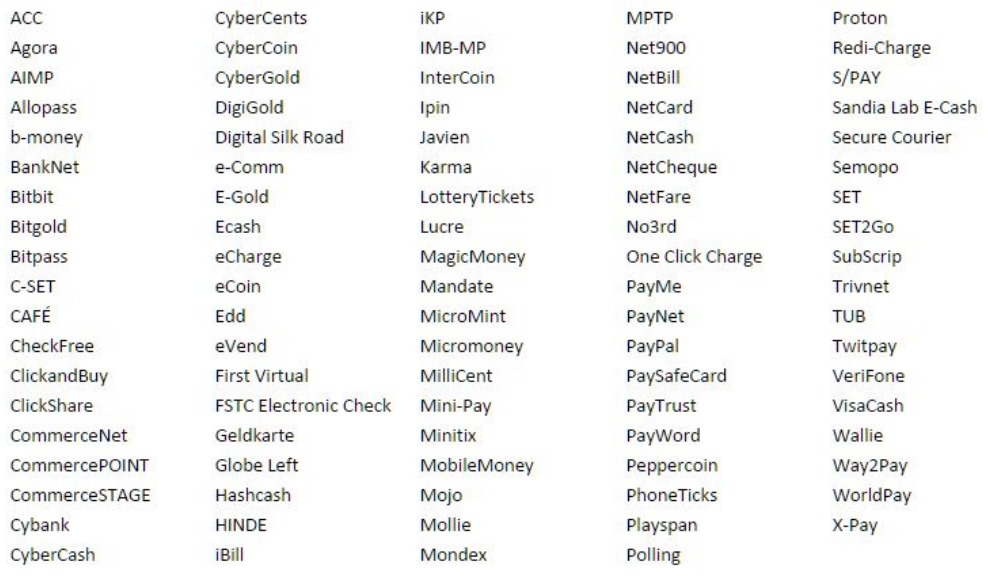
\includegraphics[width=14cm]{failedCryptos.PNG}
    \caption{Electronic payment systems before cryptocurrencies \cite{narayanan2016bitcoin}}
    \label{paymentSystems}
\end{figure}

\section{Ethereum}


\section{Bitcoin}
\begin{figure}[H]
    \centering
    \begin{lstlisting}[breaklines=true]
        >You will not find a solution to political problems in cryptography.

        Yes, but we can win a major battle in the arms race and gain a new territory of freedom for several years.
        
        Governments are good at cutting off the heads of a centrally controlled networks like Napster, but pure P2P networks like Gnutella and Tor seem to be holding their own.  
        
        Satoshi
    \end{lstlisting}
    \caption{
        Satoshi Nakamoto at vistomail.com 
        \textit{Thu Nov 6 15:15:40 EST 2008}
        % TODO fix footnote
        \protect\footnote{Archived mail from The Cryptography Mailing List 
            \url{https://www.metzdowd.com/pipermail/cryptography/2008-November/014823.html}
        }
    }
    \label{paymentSystems}
\end{figure}


\section{DigiByte}


\section{Decred}


\section{Monero}

